%%%%%%%%%%%%%%%%%%%%%%%%%%%%%%%%%%
\section{Validation of the results}
%%%%%%%%%%%%%%%%%%%%%%%%%%%%%%%%%%
%\begin{itemize}
%\item datasets
%\item definition of eta, pT bins for the different resonances
%\item description of the functions used for the fits
%\item results
%\end{itemize}
A detailed validation of the corrections and
of the smearing procedure for the 8 TeV samples was made by comparing the
position of the pole and the resolution extracted from the spectra of dimuons from
three reference resonances: J/$\psi$, $\Upsilon(1S)$ and Z. 
%Invariant mass spectra of the dimuon in 
%The models used to fit the resonances are detailed in Table~\ref{tab:fit_pdfs}.
Dimuon spectra were built in the $\eta$ and $p_T$ bins described in
Table~\ref{tab:eta_bins} and~\ref{tab:pt_bins} respectively. 
Spectra were filled if at least one muon fullfilled the
kinematic requirement, e.g. integrating over the kinematic of the
second muon.
%%%%%%%
\begin{table}[hbH]
\begin{center}
\caption{Definition of the $|\eta|$ bins used in the validation.\label{tab:eta_bins}}
\begin{tabular}{|l|cl|}
\hline
Resonance & & $|\eta|$ bin \\
\hline
J/$\psi$      &  5  $<p_T<$  7 GeV & [0,0.4] [0.4,0.8] [0.8,1.2] [1.2,1.6] [1.6,2.4] \\
              &  7  $<p_T<$ 10 GeV & [0,0.4] [0.4,0.8] [0.8,1.2] [1.2,1.6] [1.6,2.4] \\
              & 10  $<p_T<$ 15 GeV & [0,0.4] [0.4,0.8] [0.8,1.2] [1.2,1.6] [1.6,2.4] \\
\hline                    
$\Upsilon(1S)$& 10  $<p_T<$ 20 GeV & [0,0.8] [0.8,1.5] [1.5,2.4]\\
\hline                    
Z             & 20  $<p_T<$ 45 GeV & [0,0.8] [0.8,1.5] [1.5,2.1] [2.1,2.4] \\
              & 45  $<p_T<$ 90 GeV & [0,0.8] [0.8,1.5] [1.5,2.1] [2.1,2.4] \\
\hline
\end{tabular}
\end{center}
\end{table}
%%%%%%%
\begin{table}[hbH]
\begin{center}
\caption{Definition of the $p_T$ bins used in the validation.\label{tab:pt_bins}}
\begin{tabular}{|l|cl|}
\hline
Resonance & & $p_T$ bin [GeV] \\
\hline
J/$\psi$      & 0   $<|\eta|<$ 0.6 & [5,10] [10,15] [15,20] [20,25] [25,40] \\
              & 0.6 $<|\eta|<$ 1.2 & [5,10] [10,15] [15,20] [20,25] [25,40] \\
              & 1.2 $<|\eta|<$ 2.0 & [5,10] [10,15] [15,20] [20,25] [25,40] \\
\hline                     
$\Upsilon(1S)$& 0   $<|\eta|<$ 0.7 & [10,20] [20,30] \\
              & 0.7 $<|\eta|<$ 2.4 & [10,20] [20,30] \\
\hline                     
Z             & 0   $<|\eta|<$ 2.4 & [20,30] [30,40] [40,50] [50,90] \\
\hline
\end{tabular}
\end{center}
\end{table}

Figure~\ref{fig:ScaleDATAMC_8TeV} shows the fractional difference of the fitted mass
\[
\frac{M_{DATA}-M_{MC}}{M_{DATA}}
\]
as function of $|\eta|$ and  $p_T$. For the Z, the agreement is
generally much better than 0.001 in all the $|\eta|$ and $p_T$ projections.
The largest deviations are observed in the J/$\psi$ for muons at large
$\eta$ and $p_T$. These deviations are anyway below 0.001 within the
statistical error from the fit to the resonance.
\begin{figure}[hbtp]  
\begin{center}
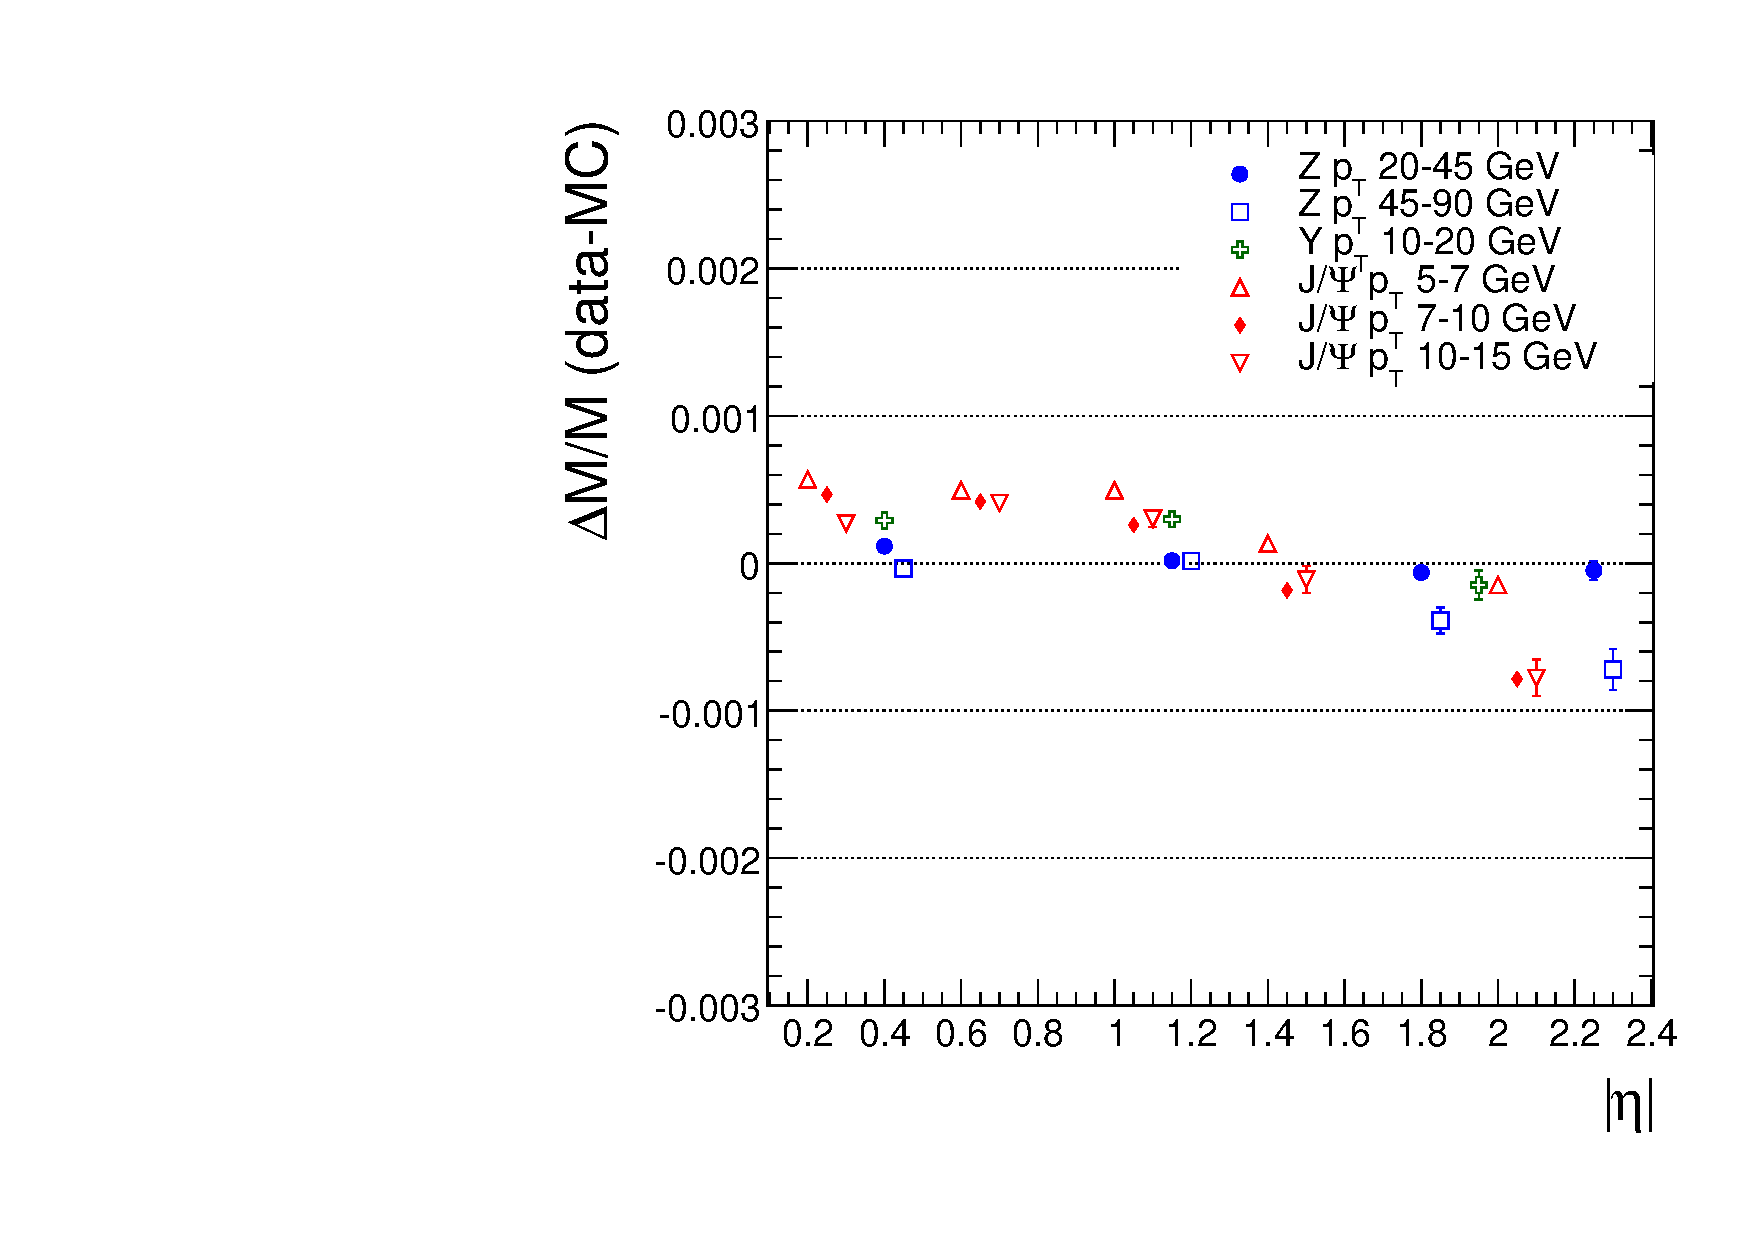
\includegraphics[width=0.7\textwidth]{figures/H4l_Style/2012_22Jan2013ReReco/ScaleEta_afterCorrection}
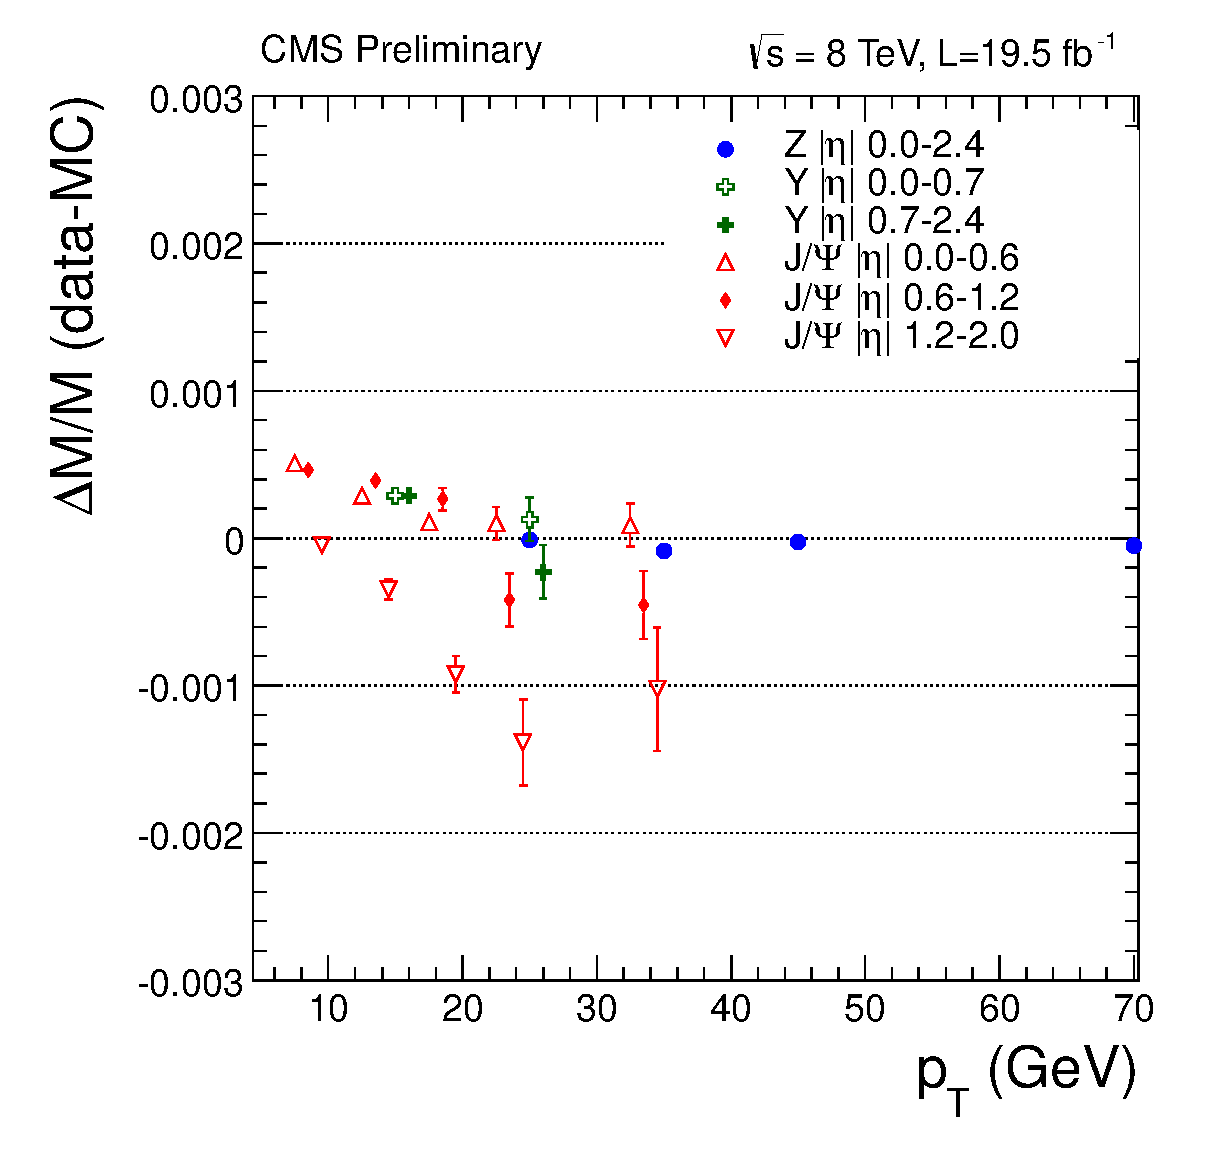
\includegraphics[width=0.7\textwidth]{figures/H4l_Style/2012_22Jan2013ReReco/ScalePt_afterCorrection} 
 \hspace{1cm} 
   \caption{Fractional difference of the fitted mass for the J/$\psi$,
     $\Upsilon(1S)$ and Z resonances as a function of the $|\eta|$ (top)
     and $p_T$ (bottom) of one of the two muons. Bars are the
     statistical error on the mass of the resonance from the fit.
   \label{fig:ScaleDATAMC_8TeV}}
 \end{center}
\end{figure} 

Figure~\ref{fig:ResolDATAMC_8TeV} shows the fractional difference of the fitted resolution.
Deviations are within $\pm$5\%.
\[
\frac{\sigma_{DATA}-\sigma_{MC}}{\sigma_{DATA}}
\]
\begin{figure}[hbtp]  
\begin{center}
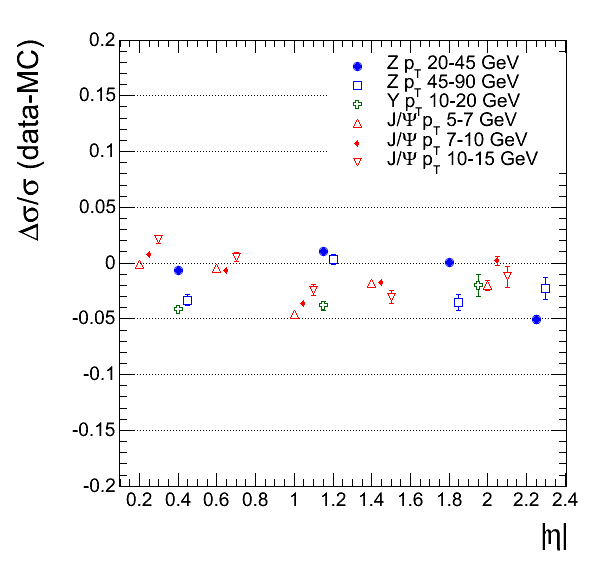
\includegraphics[width=0.7\textwidth]{figures/H4l_Style/2012_22Jan2013ReReco/ResolEta_afterCorrection}
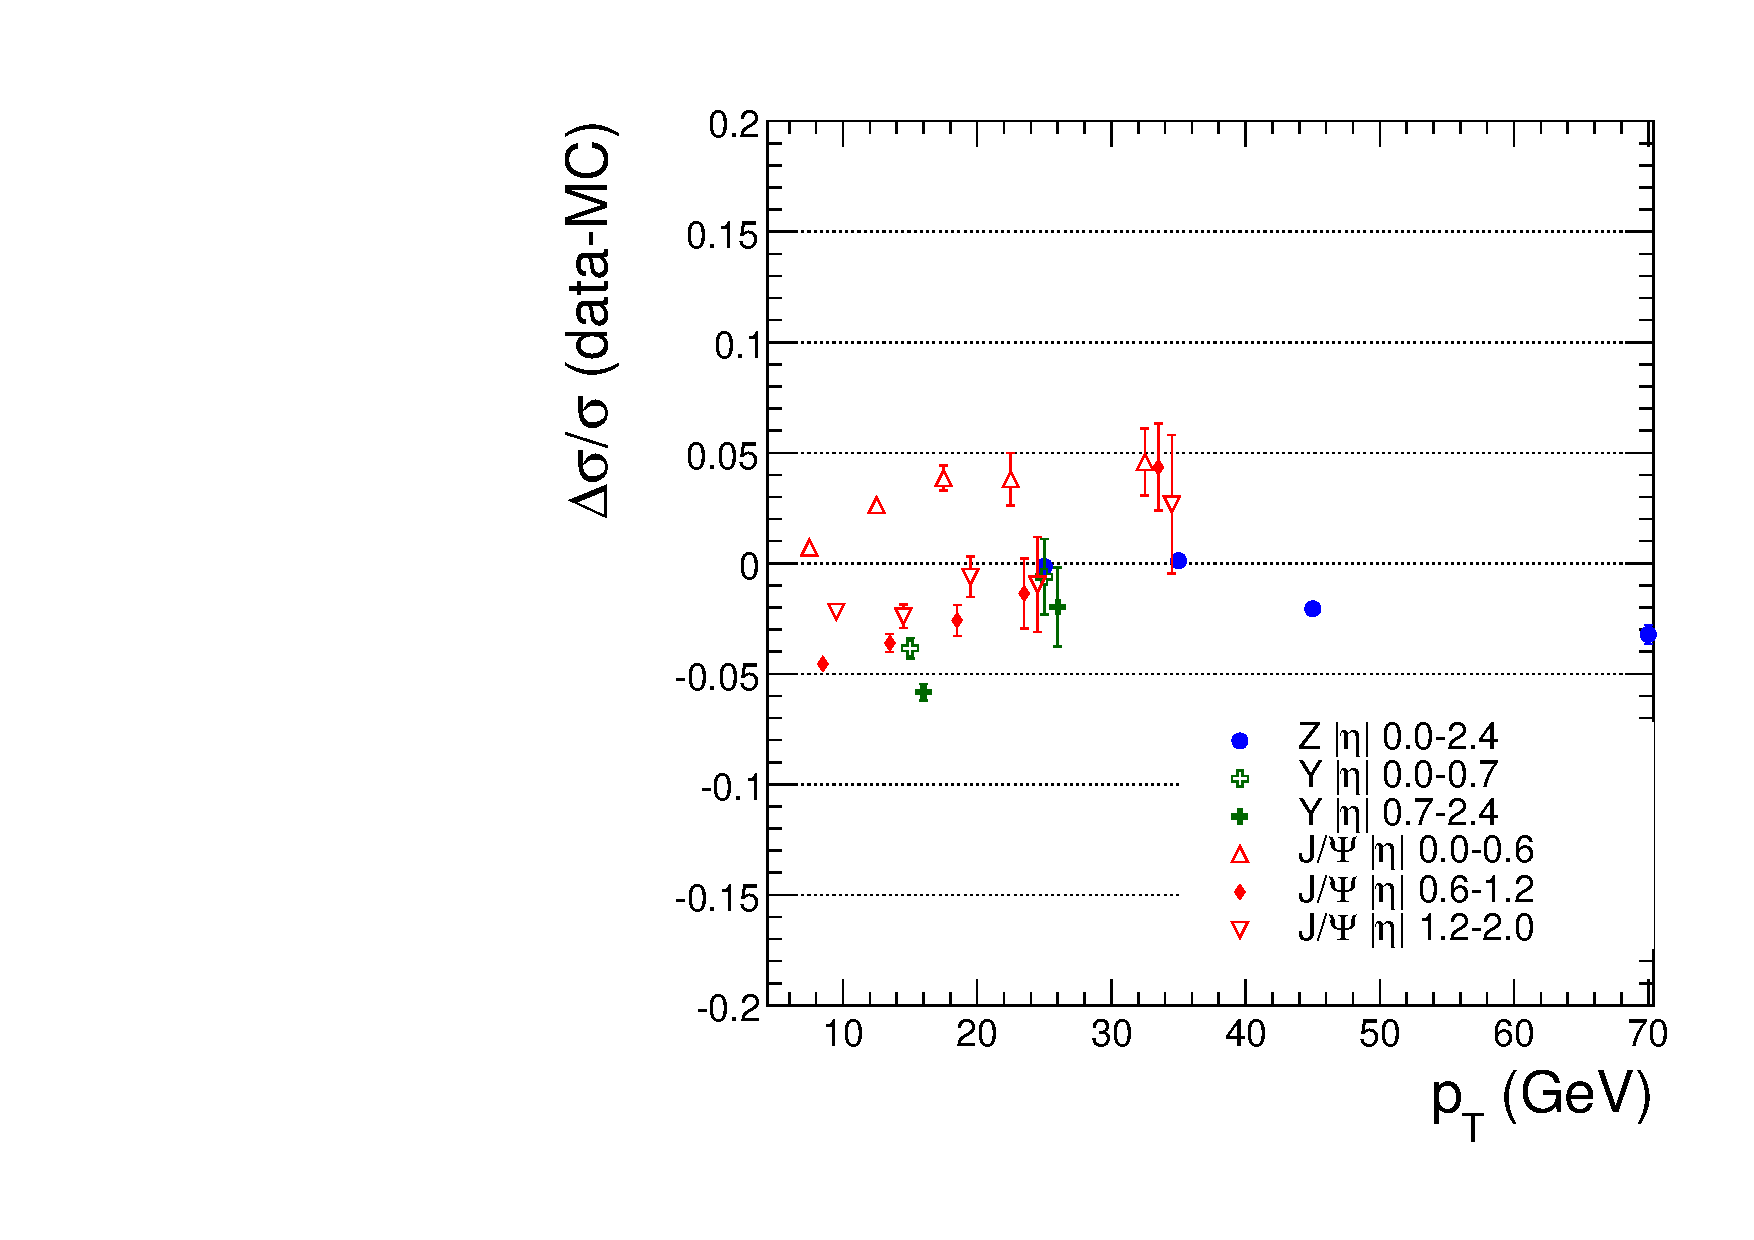
\includegraphics[width=0.7\textwidth]{figures/H4l_Style/2012_22Jan2013ReReco/ResolPt_afterCorrection} 
 \hspace{1cm} 
   \caption{Fractional difference of the fitted resolution for the J/$\psi$,
     $\Upsilon(1S)$ and Z resonances as a function of the $|\eta|$ (top)
     and $p_T$ (bottom) of one of the two muons. Bars are the
     statistical error on the resolution on the resonance from the fit.
   \label{fig:ResolDATAMC_8TeV}}
 \end{center}
\end{figure} 



